\documentclass{beamer}
\usetheme{Boadilla}
\usepackage{hyperref}
\usepackage{graphicx}
\usepackage{fancyvrb}
\usepackage{multicol}
\usepackage{adjustbox}
\usepackage{tikz}
\usetikzlibrary{shapes,positioning}
\newcommand{\foo}{\hspace{-2.3pt}$\bullet$ \hspace{5pt}}
\usepackage{subfig}
\usepackage[
    backend=biber, 
    natbib=true,
    style=numeric,
    sorting=none,
    style=verbose-ibid,
]{biblatex}
\addbibresource{citations.bib}
\usepackage{pgfpages}
\usepackage{xcolor}
\definecolor{ao(english)}{rgb}{0.0, 0.5, 0.0}
\definecolor{burgundy}{rgb}{0.5, 0.0, 0.13}
%\setbeameroption{show notes}
\setbeameroption{show notes on second screen=right}
%\setbeameroption{hide notes}

\title{The Opus Codec}
\subtitle{High-quality, low-delay music codec}
\author{Sevag Hanssian}
\date{Feburary 16, 2021}
\institute{MUMT 621, Winter 2021}
\setbeamertemplate{navigation symbols}{}

\begin{document}

\begin{frame}
\maketitle
\end{frame}

\begin{frame}
	\frametitle{Xiph.org}
	\begin{quote}
		Xiph.org is a collection of open source, multimedia-related projects.\footfullcite{xiphwebsite}
	\end{quote}
	\begin{enumerate}
			\vspace{-0.5em}
		\item
			Codecs: FLAC, Vorbis, Opus, Speex, Daala, Theora
		\item
			Misc: RNNoise (\textbf{R}ecurrent \textbf{N}eural \textbf{N}[etwork])
	\end{enumerate}
	\vspace{1em}
	\begin{quote}
		The most aggressive effort works to put the foundation standards of Internet audio and video into the public domain, where all Internet standards belong.
	\end{quote}
	\begin{enumerate}
			\vspace{-0.5em}
		\item
			Closed software and protocols are not evil or worse than open source, but by definition only exist serve the bottom line of a corporation
		\item
			 The Internet is built on open development, free exchange of ideas, and intellectual cooperation
	\end{enumerate}
\end{frame}

\note{
	\begin{itemize}
		\item
			I.e. they are not in the public's best interest
		\item
			Google AMP, facebook, twitter
		\item
			Google AMP - mention technical difficulty
		\item
			This is really becoming a problem today
	\end{itemize}
}

\begin{frame}
	\frametitle{Why multimedia needs open standards}
	\begin{enumerate}
		\item
			MPEG -- \textbf{M}oving \textbf{P}ictures \textbf{E}xpert \textbf{G}roup -- ``is the name of a family of standards used for coding audio-visual information (e.g., movies, video, music) in a digital compressed format.\footfullcite{mpegwebsite}''
		\item
			``Working group of ISO/IEC (\textbf{I}nternational \textbf{O}rganization for \textbf{S}tandardization, \textbf{I}nternational \textbf{E}lectrotechnical \textbf{C}ommission) in charge of the development of international standards for compression, decompression, processing, and coded representation of moving pictures, audio and their combination.''
		\item
			RIAA -- \textbf{R}ecording \textbf{I}ndustry \textbf{A}ssociation of \textbf{A}merica -- \footfullcite{riaaweb}
			\begin{quote}
				We work to protect artists' creative freedom and promote the unique work that labels do to support them. [...] We work to protect artists and all music creators from the damaging impact of music theft. 
			\end{quote}
	\end{enumerate}
\end{frame}

\begin{frame}
	\frametitle{MP3 in 1998}
	Fraunhofer/Thompson (two industrial giants holding MP3-related patents) started demanding royalties in 1998\footfullcite{computall}:
	\begin{quote}
		Since 1997, we have been working with the MP3 source code released by the ISO. [...] Then we got an e-mail [...] ``As you may know, both the Fraunhofer Institute and THOMSON have done important work to develop MPEG Layer-3 audio compression (before and after it became part of the MPEG standards). This work has resulted in many inventions and several patents, covering the MPEG Layer-3 standard. Our files do not show that you have a valid license agreement with us. This means that the products infringe the patent rights of Fraunhofer and THOMSON.''
	\end{quote}
	RIAA sued an MP3 player manufacturer, Diamond, in the late 90s\footfullcite{riaavdiamond}
\end{frame}

\note{
	\begin{itemize}
		\item
			story of computall
		\item
			two forms of evil here
			\begin{itemize}
				\item
					corporate giants who pretend to develop open standards, then apply a royalty
				\item
					music publishers who are terrified of open standards
			\end{itemize}
		\item
			birth of vorbis right here
	\end{itemize}
}

\begin{frame}
	\frametitle{Containers and codecs}
	\begin{enumerate}
		\item
			A \textit{container} is associated to the file extension -- it describes which codecs are used for its video/audio contents, followed by the actual encoded video/audio data, and extra data such as subtitles
		\item
			A \textit{codec} defines how to \textit{encode} raw audio/video into data to put in a container (i.e. file), and how to \textit{decode} data from the container back to a form suitable for playback\footfullcite{pitivi}
	\end{enumerate}
	\begin{table}[ht]
	\centering
	\begin{tabular}{llll c c c c}
		\hline\hline
		File extension & Audio codec & Video codec & Container \\ [0.5ex]
		\hline\hline
		.webm & Vorbis or Opus & VP8 or VP9 & Matroska \\ [0.5ex]
		.mkv & Any & Any & Matroska \\ [0.5ex]
		.ogg & Vorbis & n/a & Ogg \\ [0.5ex]
		.opus & Opus & n/a & Ogg \\ [0.5ex]
		.mp4 & AAC & MPEG-4 & MP4 \\ [0.5ex]
		\hline
	\end{tabular}
	\end{table}
\end{frame}

\begin{frame}
	\frametitle{The Opus Codec}
	Audio codec designed for the Internet\footfullcite{opuspaper}
	\begin{itemize}
		\item
			Open-source, royalty-free
		\item
			Lossy
		\item
			Can trade off quality to reduce latency
		\item
			Derives from:
			\begin{itemize}
				\item
					CELT (\textbf{C}onstrained-\textbf{Energy} and \textbf{L}apped \textbf{T}ransform)
				\item
					SILK, Skype speech codec
			\end{itemize}
		\item
			Replaces Vorbis (music) and Speex (speech) in a single codec
	\end{itemize}
	Opus can operate in three modes:
	\begin{enumerate}
		\item
			SILK mode for speech -- low bitrate narrowband speech
		\item
			CELT mode for music -- high bitrate, high quality music
		\item
			Hybrid -- SILK <8kHz, CELT >8kHz
	\end{enumerate}
\end{frame}

\note{
\begin{itemize}
	\item
		SILK is not an acronym
	\item
		CELT used to be a standalone algorithm, derived from Vorbis, now its the music part of opus
	\item
		It can change modes within a stream -- making it good for some degradation that occurs as the internet gets choppy
	\item
		8khz? segue into speech v music
\end{itemize}
}

\begin{frame}
	\frametitle{Speech and music}
	\begin{table}[ht]
	\centering
	\begin{tabular}{lll c c c}
		\hline\hline
		Sampling rate (Hz) & Max frequency (Hz) & Name \\ [0.5ex]
		\hline\hline
		8000 & 4000 & Narrowband \\ [0.5ex]
		16000 & 8000 & Wideband \\ [0.5ex]
		\hline
		44100 & 22050 & CD \\ [0.5ex]
		48000 & 24000 & Fullband (DVD) \\ [0.5ex]
		\hline
	\end{tabular}
	\end{table}
	80\% of perceptually important spectrum in \textit{voiced} speech is <4kHz, however speech up to 8kHz is preferred in subjective tests (due to \textit{unvoiced} speech)\footfullcite{speech}. Humans can hear from 20Hz-20kHz, and music requires a larger frequency range than speech\footfullcite{moore}.
\end{frame}

\note{
	\begin{itemize}
		\item
			Refresher on the Nyquist frequency: Audio sampled at X kHz can only contain frequencies up to $\frac{X}{2}$ kHz

		\item
			Omitted 12000, 6000 which is mediumband and 24000/12000 which is superwideband
		\item
			32000, 16000, nb cassette's are analog but they can't contain more than 18000hz
		\item
			Voiced signals are produced when the vocal cords vibrate during the pronounciation of a phoneme
		\item
			Unvoiced signals, by contrast, do not entail the use of the vocal cords
		\item
			f versus v, s versus z
		\item
			There is 96000, ultrasonic - supporting frequencies up to 48000 hz. not useful for humans
	\end{itemize}
}

\begin{frame}
	\frametitle{Lossy compression and psychoacoustics}
	\textit{Lossy} versus \textit{lossless} encoding is the primary issue in data compression\footfullcite{skiena}
	Lossy compression sacrifices data for space savings\\\ \\
	A question of fidelity: can we perceive the lost data? In the case of audio encoding, we need to consider psychoacoustics and perception.
	\begin{quote}
		The basis of lossy psychoacoustical compression methods is the omission of information from the audio signal so that it does not result in perceived difference.\footfullcite{lossypsycho}
	\end{quote}
	\href{https://wiki.xiph.org/Opus_Recommended_Settings}{https://wiki.xiph.org/Opus\_Recommended\_Settings} says to prefer FLAC (lossless) for archival to avoid generation loss\footfullcite{generationloss}
\end{frame}

\begin{frame}
	\adjustbox{valign=c}{{\usebeamerfont{frametitle}\usebeamercolor[fg]{frametitle}Opus timeline}}\hfill
	\adjustbox{valign=c}{
	\newcounter{year}
	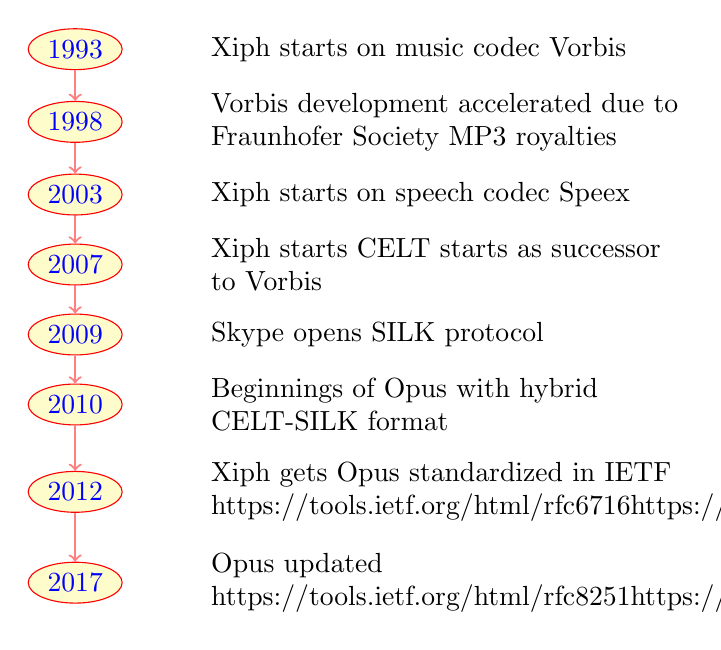
\begin{tikzpicture}[yscale=0.5,%
		   year/.style={draw=red,text=blue,fill=yellow!20,shape=ellipse,inner sep=2pt},
		   description/.style={rectangle,align=left,text width=60mm,anchor=west},
		   timeline/.style={->,thick,red!50}]

	    \foreach \year/\desc [count=\y] in {%
	       1993/Xiph starts on music codec Vorbis,%
	       1998/Vorbis development accelerated due to Fraunhofer Society MP3 royalties,%
	       2003/Xiph starts on speech codec Speex,%
	       2007/Xiph starts CELT starts as successor to Vorbis,%
	       2009/Skype opens SILK protocol,%
	       2010/Beginnings of Opus with hybrid CELT-SILK format,%
		2012/Xiph gets Opus standardized in IETF \href{https://tools.ietf.org/html/rfc6716}{https://tools.ietf.org/html/rfc6716},%
		2017/Opus updated \href{https://tools.ietf.org/html/rfc8251}{https://tools.ietf.org/html/rfc8251}%
	       } { \ifnum\y=1 \node[description](\y){\desc};
		   \else\node[description,below=1ex of \z](\y){\desc};
		   \fi
		   \node[year](y-\y) [left=of \y] {\year};
		   \ifnum\y>1\draw[timeline] (y-\z)-- (y-\y);\fi
		   \global\let\z=\y% for drawing from last node
	       }

	\end{tikzpicture}
	}
\end{frame}

\note{
\begin{itemize}
	\item
		skype works with xiph and others to get something SILK-like in IETF - ultimately opus is the one who wins in IETF
	\item
		vorbis officially deprecated for opus
	\item
		speex is more softly discouraged. but not as strongly
\end{itemize}
}

\begin{frame}
	\frametitle{Opus details -- speech}
	The SILK half of Opus:\footfullcite{opuspapervoice}:
	\begin{itemize}
		\item
			\textit{for speech, linear prediction techniques, such as Code-Excited Linear Prediction (CELP), code low frequencies more efficiently than transform (e.g., MDCT) domain techniques}
		\item
			Based on LPC (\textbf{L}inear \textbf{P}redictive \textbf{C}oding). Larynx emits simple signal (white noise or impulse train) through the articulatory system (throat, etc.) with coefficients. Sender sends articulatory coefficients, receiver recreates original sound by driving larynx signal through it\footfullcite{larynx}
		\item
			Computes LPC coefficients for \textit{voiced} and \textit{unvoiced} speech differently, using results of pitch analysis
	\end{itemize}
\end{frame}

\note{
	\begin{itemize}
		\item
			LPC is hugely popular in speech
		\item
			To make a musical analogy, it's like listening to a piano performance, transcribing it, sending over the score, and getting someone to play it on the other end... The result on the other end will be close to the original performance, but only a representation has been sent over.
	\end{itemize}
}

\begin{frame}
	\frametitle{Opus details -- music}
	The CELT half of Opus:\footfullcite{opuspaper}:
	\begin{itemize}
		\item
			Based on MDCT (\textbf{M}odified \textbf{D}iscrete \textbf{C}osine \textbf{T}transform). The DFT (\textbf{D}iscrete \textbf{F}ourier \textbf{T}ransform) decomposes a real acoustic signal into a sum of complex exponentials. The DCT uses only real cosines, and spectral energy is concentrated in fewer coefficients than the DFT\footfullcite{dct}.
		\item
			In addition to MDCT coefficients, CELT includes information about the spectral envelope of the signal with energy in Bark-like bands:
	\end{itemize}
	\begin{figure}
	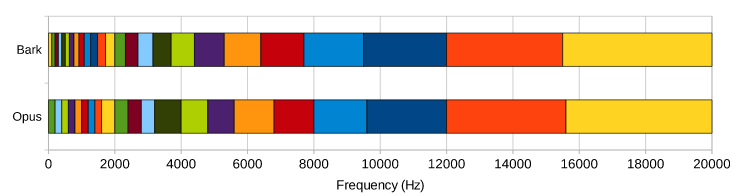
\includegraphics[width=8cm]{./bark.png}
	\end{figure}
\end{frame}

\note{
	\begin{itemize}
		\item
			like lpc is dominant for speech, mdct is dominant for audio codecs
		\item
			lots of DCTs, details were too much to get into
		\item
			fewer coefficients means that the DCT is very used in compression
	\end{itemize}
}

\begin{frame}
	\frametitle{Auto-detect music and speech}
	Opus can automatically detect whether its input is speech or music, and choose the optimal encoding mode accordingly. GRU (\textbf{G}ated \textbf{R}ecurrent \textbf{U}nit) with just 4986 weights (that fit in less than 5 kB) and takes about 0.02\% CPU to run in real-time\footfullcite{valinopus}
	\begin{figure}
	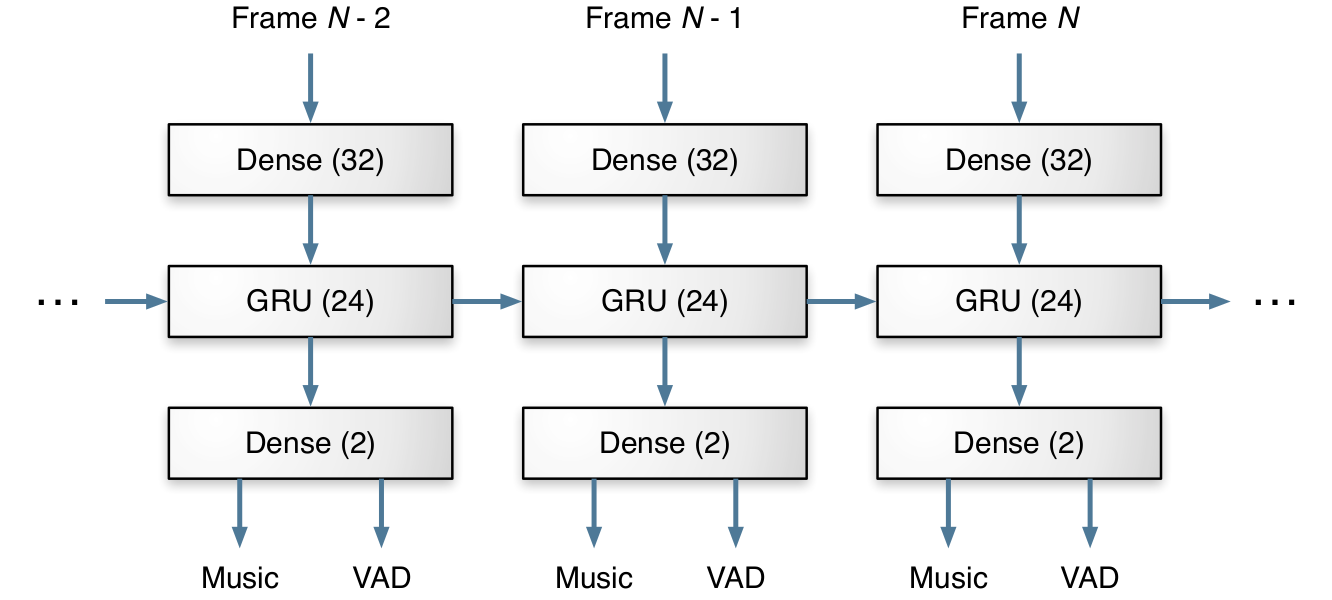
\includegraphics[width=9cm]{./opus_gru.png}
	\end{figure}
\end{frame}

\begin{frame}
	\frametitle{Ambisonics, spatial audio}
	\begin{quote}
		Opus 1.3 adds support for immersive audio using ambisonics that surrounds the listener in a full-sphere sound field. This is done through two new (soon to be RFC 8486) Ogg mapping families for Opus ambisonics. Unlike other multi-channel surround formats, ambisonics is independent of speaker layout. This allows for flexible speaker configurations and scalable audio to efficiently transmit 3D audio soundtracks.\footfullcite{valinopus}
	\end{quote}
	\href{https://tools.ietf.org/html/rfc8486}{https://tools.ietf.org/html/rfc8486}
\end{frame}

\note{
	\begin{itemize}
		\item
			jake mentioned
		\item
			note that the change is to Ogg, the container, to include multiple ambisonic channels of Opus-encoded audio
	\end{itemize}
}

\begin{frame}
	\frametitle{Sound samples}
	\href{https://opus-codec.org/examples/}{https://opus-codec.org/examples/}
\end{frame}

\end{document}
